\documentclass[12pt]{aghdpl}
% \documentclass[en,11pt]{aghdpl}  % praca w języku angielskim

% Lista wszystkich języków stanowiących języki pozycji bibliograficznych użytych w pracy.
% (Zgodnie z zasadami tworzenia bibliografii każda pozycja powinna zostać utworzona zgodnie z zasadami języka, w którym dana publikacja została napisana.)
\usepackage[english,polish]{babel}

% Użyj polskiego łamania wyrazów (zamiast domyślnego angielskiego).
\usepackage{polski}

\usepackage[utf8]{inputenc}

% dodatkowe pakiety

\usepackage{mathtools}
\usepackage{amsfonts}
\usepackage{amsmath}
\usepackage{amsthm}

% --- < bibliografia > ---

\usepackage[
style=numeric,
sorting=none,
%
% Zastosuj styl wpisu bibliograficznego właściwy językowi publikacji.
language=autobib,
autolang=other,
% Zapisuj datę dostępu do strony WWW w formacie RRRR-MM-DD.
urldate=edtf,
% Nie dodawaj numerów stron, na których występuje cytowanie.
backref=false,
% Podawaj ISBN.
isbn=true,
% Nie podawaj URL-i, o ile nie jest to konieczne.
url=false,
%
% Ustawienia związane z polskimi normami dla bibliografii.
maxbibnames=3,
% Jeżeli używamy BibTeXa:
backend=bibtex
]{biblatex}

\usepackage{csquotes}
% Ponieważ `csquotes` nie posiada polskiego stylu, można skorzystać z mocno zbliżonego stylu chorwackiego.
\DeclareQuoteAlias{croatian}{polish}

\addbibresource{bibliografia.bib}

% Nie wyświetlaj wybranych pól.
%\AtEveryBibitem{\clearfield{note}}


% ------------------------
% --- < listingi > ---

% Użyj czcionki kroju Courier.
\usepackage{courier}

\usepackage{listings}
\lstloadlanguages{TeX}

\lstset{
	literate={ą}{{\k{a}}}1
           {ć}{{\'c}}1
           {ę}{{\k{e}}}1
           {ó}{{\'o}}1
           {ń}{{\'n}}1
           {ł}{{\l{}}}1
           {ś}{{\'s}}1
           {ź}{{\'z}}1
           {ż}{{\.z}}1
           {Ą}{{\k{A}}}1
           {Ć}{{\'C}}1
           {Ę}{{\k{E}}}1
           {Ó}{{\'O}}1
           {Ń}{{\'N}}1
           {Ł}{{\L{}}}1
           {Ś}{{\'S}}1
           {Ź}{{\'Z}}1
           {Ż}{{\.Z}}1,
	basicstyle=\footnotesize\ttfamily,
}

% ------------------------

\AtBeginDocument{
	\renewcommand{\tablename}{Tabela}
	\renewcommand{\figurename}{Rys.}
}

% ------------------------
% --- < tabele > ---

\usepackage{array}
\usepackage{tabularx}
\usepackage{multirow}
\usepackage{booktabs}
\usepackage{makecell}
\usepackage[flushleft]{threeparttable}

% defines the X column to use m (\parbox[c]) instead of p (`parbox[t]`)
\newcolumntype{C}[1]{>{\hsize=#1\hsize\centering\arraybackslash}X}


%---------------------------------------------------------------------------

\author{Michał Gandor}
\shortauthor{M. Gandor}

%\titlePL{Przygotowanie bardzo długiej i pasjonującej pracy dyplomowej w~systemie~\LaTeX}
%\titleEN{Preparation of a very long and fascinating bachelor or master thesis in \LaTeX}

\titlePL{Symulacja dynamiki pieszych z wykorzystaniem modelu Social Force.}
\titleEN{Simulation of pedestrian dynamics using Social Force Model.  }

\thesistype{Praca dyplomowa inżynierska}
%\thesistype{Master of Science Thesis}

\supervisor{dr hab. inż. Jarosław Wąs}
%\supervisor{Marcin Szpyrka PhD, DSc}

\degreeprogramme{Informatyka}
%\degreeprogramme{Computer Science}

\date{2017}

\department{Katedra Informatyki Stosowanej}
%\department{Department of Applied Computer Science}

\faculty{Wydział Elektrotechniki, Automatyki,\protect\\[-1mm] Informatyki i Inżynierii Biomedycznej}
%\faculty{Faculty of Electrical Engineering, Automatics, Computer Science and Biomedical Engineering}

\acknowledgements{Serdecznie dziękuję \dots tu ciąg dalszych podziękowań np. dla promotora, żony, sąsiada itp.}


\setlength{\cftsecnumwidth}{10mm}

%---------------------------------------------------------------------------
\setcounter{secnumdepth}{4}
\brokenpenalty=10000\relax

\begin{document}

\titlepages

% Ponowne zdefiniowanie stylu `plain`, aby usunąć numer strony z pierwszej strony spisu treści i poszczególnych rozdziałów.
\fancypagestyle{plain}
{
	% Usuń nagłówek i stopkę
	\fancyhf{}
	% Usuń linie.
	\renewcommand{\headrulewidth}{0pt}
	\renewcommand{\footrulewidth}{0pt}
}

\setcounter{tocdepth}{2}
\tableofcontents
\clearpage

\chapter{Wprowadzenie}
\label{cha:wprowadzenie}

Zachowanie tłumu badane jest od przeszło trzech dekad. Na samym początku badania były traktowane w ramach ciekawostki. Wraz z nowatorskimi pracami Helbinga .... . W ostatnich latach zagadnienie to zyskuje coraz większe znaczenie. Jesteśmy obecnie świadkami rozrostu miast, budowy kompleksów sportowych czy galerii handlowych. Wszystkie te miejsca są nieodłącznie związane z tłumami przewijających się przez nie osób. W związku z rosnącą gęstością zaludnienia oraz wzrostem zagoreń takich jak terroryzm [jakis przypis] tworzenie symulacji ewakuacji nabrało większego znaczenia. Dzięki zasymulowaniu zachowania tłumu możenmy łatwiej utworzyć schematy opuszczenia bynków podczaz zagorżenia minimaliusjąc szkody oraz ofiary. Symulacje pozwalają także na lepsze rozładowanie ruchu drogowego w miastach o roznącej ilości zaludnienia.

Symulacje mogą mieć wielorakie zastosowanie, począwszy od ewakucaji ludności poprzez zachowania w centrach handlowych kończąc na ruchu drogowym. Na przejściach dla pieszych w Japonii ginie 30\% osób uczestniczących w wypadkach drogowych \cite{AMSFMfPBSaSC}, a w Niemczech odsetek ten wynosi 15\% \ [German instigute for econeomic research 2010]. Zgodnie z danymi organizacjie Fire Administration w Stanach Zjednoczonych \cite{Asfemwle} w roku 2007 3430 osób zmarło w pożarach oraz blisko 18 tysięcy zostało ranych.

%---------------------------------------------------------------------------

\section{Cele pracy}
\label{sec:celePracy}

Celem poniższej pracy jest zapoznanie studentów z systemem \LaTeX~w zakresie umożliwiającym im samodzielne, profesjonalne złożenie pracy dyplomowej w systemie \LaTeX.

%---------------------------------------------------------------------------

\section{Zawartość pracy}
\label{sec:zawartoscPracy}

W rodziale~\ref{cha:pierwszyDokument} przedstawiono podstawowe informacje dotyczące struktury dokumentów w \LaTeX u. Alvis~\cite{Alvis2011} jest językiem 



















\chapter{Wykaz ważniejszych oznaczeń}
\label{sec:wykazOznaczen}

SFM - Social Force Model
A* - algorytm A Star
POI - points of intrests
[do dopisania]

















\chapter{Wprowadzenie teoretyczne}
\label{cha:wprowadzenieTeoretyczne}

Dziedziny nauki badające ruch pieszych to nie tylko informatyka. Na powstanie modeli miały także wpływ prace uczonych z takich dziedzin jak psychologia, socjologia czy architektura. Problem zachowania tłumu jest skomplikowany i dopiero połączenie tych wszystkich dziedzin dało początek realnemu odzwierciedleniu na ekranie komputera. \\
Z pozoru zachowanie pieszych może wydawać się chaotyczne oraz trudne do przewidzenia. Bazując jednak na badaniach i obserwacjach takie zachowania mają miejsce tylko w skrajnych przypadkach. W codziennym życiu okazuje się, że model do opisu zachowania tłumu może być w dość prosty sposób opisany, głównie dzięki prawdopodobieństwom jakie mogą zostać nakreślone w dużych populacjach ludzi. Człowiek ma tendencję do podejmowania decyzji na bazie posiadanej już wcześniej, wypracowanej wiedzy na temat otaczającego go środowiska. Oznacza to, że reakcje na innych pieszych oraz przeszkody mogą być w łatwy sposób przewidziane. Analogią do takiego zachowania mogą być przykładowo reakcje profesjonalnego kierowcy wyścigowego, który reaguje na sytuacje drogowe niemal automatycznie.

Oczywiście nie jest to prawdą w każdej sytuacji. Przykładowo dzieci oraz turyści wykazują inny sposób poruszania się za względu na to, że zazwyczaj znajdują się w nowym miejscu i nie mają wypracowanej strategii poruszania się. Jednakże dla potrzeb symulacji nie potrzeba dokładnych informacji o każdym z pieszych. W zupełności wystarcza statystyczna wartość konkretnych zachowań

W tym rozdziale zostają przedstawione podstawowe dostępne obecnie modele. Każdy z modeli ma swoje zalety oraz wady, wpływają na to cechy takie jak złożoność obliczeniowa, złożoność implementacji oraz oczywiście cechy otrzymanych rezultatów.

\section{Klasyfikacja modeli symulacji ruchu pieszych}
\label{sec:klasyfikacja}

\subsection{Modele mikroskopowe oraz makrospokope}

Modele makroskopowe pokazują w głównej mierze dynamikę gęstości oraz prędkości całego tłumu. W tym celu używane są istniejące już modele fizyczne takie jak dynamika płynów, które zostają odpowiednio dostosowane do potrzeb symulacji. Przykładem może być hydrodynamiczny model Paulusa opierający się na równaniach przepływu \cite{ArchitekturaModelowania}. Modele te nie biorą pod uwagę indywidualnych zachowań jednostki.\\

Podejście makrospokowe ze względu na odzwierciedlanie całej populacji sprawdza się w praktyce tylko w wąskim wachlarzu zastosowań.
 
Jako zaletę podejścia makroskopowego możemy z pewnością wskazać mniejszą ilość obliczeń potrzebną do uzyskania porządanego efektu.

Modele mikrospokowe, w przeciwieństwie do wspomnianych wyżej modeli makroskopowych, biorą one pod uwagę zachowanie konkretnej jednostki. Badane są interakcje pomiędzy pieszymi oraz ich iteracje z przeszkodami oraz otaczającą rzeczywistością. Modele te pozwalają na uzyskanie efekty bardziej odpowiadającego realnemu zachowaniu tłumu. Jednakże wraz ze wzrostem odwzorowania detali wzrasta również złożoność systemu oraz zwiększa się złożoność obliczeń co skutkuje toeretycznie gorszą wydajnością, jednak przy dostępnej obecnie mocy obliczeniowej nawet standardowych komputerów nie gra to aż takiej roli.

\subsection{Modele ciągłe i dyskretne}

W modelach mikroskopowych możemy wyodrębinić dwie podgrupy: modele ciągłe oraz dyskretne. Modele dyskretne cechują się zmianą paramatrów stanu w konkretnych interwałąch czasowych, przyjmują okręślone wartości dla określonych argumantów i tylko dla nich. W modelach ciągłych stan ulega zmienie przez cały czas działania, może przyjmować dowonlą wartość z całego przedziału. Modele ciągłe reprezentują oczywiście dane w sposób bardziej realistyczny, jednakże zwiększają czas obliczeń \\

Jednym z przykładów na model dyskretny może być automat komórkowy. Uniwersalność automatów komórkowych \textit{Cellular Automata} spowodowała, iż znajdują zastosowanie także w dziedzinie symulacji ruchu pieszych. Automat komórkowy jest modelem matematycznym, który specyfikuje siatka komórek, zbiór stanów jakie mogą one przyjmować, oraz reguły określające stan komórki w chwili $t + 1$. Stan danej komórki zależny jest od stanu komórek z nią sąsiadujących w chwili $t$. \\

Dla stworzenia modeli mikroskopowych używano z początku niehomogenicznych automatów komórkowych. Wraz z rozwojem symulacji na automatach komórkowych można było dostrzec duże zmiany bazowym modelu. Powstające symulacje zaczęły zostać klasyfikowane jako \textbf{sytemy agentowe}.

Niestety jednorodność tej metody uniemożliwia modelowanie bardziej skomplikowanych procesów\cite{FormalizacjaAutomatów}.

%---------------------------------------------------------------------------



















\chapter{Przykłady elementów pracy dyplomowej}

\section{Liczba}

Pakiet \texttt{siunitx} zadba o to, by liczba została poprawnie sformatowana: \\
\begin{center}
	\num{1234567890.0987654321}
\end{center}


\section{Rysunek}

Pakiet \texttt{subcaption} pozwala na umieszczanie w podpisie rysunku odnośników do ,,podilustracji'': \\

\begin{figure}[h]
	\centering
	\begin{subfigure}{0.35\textwidth}
		\centering
		\framebox[2.0\width]{A}
		\subcaption{\label{subfigure_a}}
	\end{subfigure}
	\begin{subfigure}{0.35\textwidth}
		\centering
		\framebox[2.0\width]{B}
		\subcaption{\label{subfigure_b}}
	\end{subfigure}
	
	\caption{\label{fig:subcaption_example}Przykład użycia \texttt{\textbackslash subcaption}: \protect\subref{subfigure_a} litera A, \protect\subref{subfigure_b} litera B.}
\end{figure}

\section{Tabela}

Pakiet \texttt{threeparttable} umożliwia dodanie do tabeli adnotacji: \\

\begin{table}[h]
	\centering
	
	\begin{threeparttable}
		\caption{Przykład tabeli}
		\label{tab:table_example}
		
		\begin{tabularx}{0.6\textwidth}{C{1}}
			\toprule
			\thead{Nagłówek\tnote{a}} \\
			\midrule
			Tekst 1 \\
			Tekst 2 \\
			\bottomrule
		\end{tabularx}
		
		\begin{tablenotes}
			\footnotesize
			\item[a] Jakiś komentarz\textellipsis
		\end{tablenotes}
		
	\end{threeparttable}
\end{table}

\section{Wzory matematyczne}

Czasem zachodzi potrzeba wytłumaczenia znaczenia symboli użytych w równaniu. Można to zrobić z użyciem zdefiniowanego na potrzeby niniejszej klasy środowiska \texttt{eqwhere}.

\begin{equation}
E = mc^2
\end{equation}
gdzie
\begin{eqwhere}[2cm]
	\item[$m$] masa
	\item[$c$] prędkość światła w próżni
\end{eqwhere}

Odległość półpauzy od lewego marginesu należy dobrać pod kątem najdłuższego symbolu (bądź listy symboli) poprzez odpowiednie ustawienie parametru tego środowiska (domyślnie: 2 cm).

\chapter{Pierwszy dokument}
\label{cha:pierwszyDokument}

W rozdziale tym przedstawiono podstawowe informacje dotyczące struktury prostych plików \LaTeX a. Omówiono również metody kompilacji plików z zastosowaniem programów \emph{latex} oraz \emph{pdflatex}.

%---------------------------------------------------------------------------

\section{Struktura dokumentu}
\label{sec:strukturaDokumentu}

Plik \LaTeX owy jest plikiem tekstowym, który oprócz tekstu zawiera polecenia formatujące ten tekst (analogicznie do języka HTML). Plik składa się z dwóch części:
\begin{enumerate}%[1)]
\item Preambuły -- określającej klasę dokumentu oraz zawierającej m.in. polecenia dołączającej dodatkowe pakiety;

\item Części głównej -- zawierającej zasadniczą treść dokumentu.
\end{enumerate}


\begin{lstlisting}
\documentclass[a4paper,12pt]{article}      % preambuła
\usepackage[polish]{babel}
\usepackage[utf8]{inputenc}
\usepackage[T1]{fontenc}
\usepackage{times}

\begin{document}                           % część główna

\section{Sztuczne życie}

% treść
% ąśężźćńłóĘŚĄŻŹĆŃÓŁ

\end{document}
\end{lstlisting}

Nie ma żadnych przeciwskazań do tworzenia dokumentów w~\LaTeX u w~języku polskim. Plik źródłowy jest zwykłym plikiem tekstowym i~do jego przygotowania można użyć dowolnego edytora tekstów, a~polskie znaki wprowadzać używając prawego klawisza \texttt{Alt}. Jeżeli po kompilacji dokumentu polskie znaki nie są wyświetlane poprawnie, to na 95\% źle określono sposób kodowania znaków (należy zmienić opcje wykorzystywanych pakietów).


%---------------------------------------------------------------------------

\section{Kompilacja}
\label{sec:kompilacja}


Załóżmy, że przygotowany przez nas dokument zapisany jest w pliku \texttt{test.tex}. Kolejno wykonane poniższe polecenia (pod warunkiem, że w pierwszym przypadku nie wykryto błędów i kompilacja zakończyła się sukcesem) pozwalają uzyskać nasz dokument w formacie pdf:
\begin{lstlisting}
latex test.tex
dvips test.dvi -o test.ps
ps2pdf test.ps
\end{lstlisting}
%
lub za pomocą PDF\LaTeX:
\begin{lstlisting}
pdflatex test.tex
\end{lstlisting}

Przy pierwszej kompilacji po zmiane tekstu, dodaniu nowych etykiet itp., \LaTeX~tworzy sobie spis rozdziałów, obrazków, tabel itp., a dopiero przy następnej kompilacji korzysta z tych informacji.

W pierwszym przypadku rysunki powinny być przygotowane w~formacie eps, a~w~drugim w~formacie pdf. Ponadto, jeżeli używamy polecenia \texttt{pdflatex test.tex} można wstawiać grafikę bitową (np. w formacie jpg).



%---------------------------------------------------------------------------

\section{Narzędzia}
\label{sec:narzedzia}


Do przygotowania pliku źródłowego może zostać wykorzystany dowolny edytor tekstowy. Niektóre edytory, np. GEdit, mają wbudowane moduły ułatwiające składanie tekstów w LaTeXu (kolorowanie składni, skrypty kompilacji, itp.).

Jednym z bardziej znanych środowisk do składania dokumentów  \LaTeX a jest {\em TeXstudio}, oferujące kompletne środowisko pracy. Zobacz: \url{http://www.texstudio.org}


Bardzo dobrym środowiskiem jest również edytor gEdit z wtyczką obsługującą \LaTeX a. Jest to standardowy edytor środowiska Gnome. Po instalacji wtyczki obsługującej \LaTeX~ zamienia się w wygodne i szybkie środowisko pracy.

\textbf{Dla testu łamania stron powtórzenia powyższego tekstu.}


Do przygotowania pliku źródłowego może zostać wykorzystany dowolny edytor tekstowy. Niektóre edytory, np. GEdit, mają wbudowane moduły ułatwiające składanie tekstów w LaTeXu (kolorowanie składni, skrypty kompilacji, itp.).
Jednym z bardziej znanych środowisk do składania dokumentów  \LaTeX a jest {\em TeXstudio}, oferujące kompletne środowisko pracy. Zobacz: \url{http://www.texstudio.org}
Bardzo dobrym środowiskiem jest również edytor gEdit z wtyczką obsługującą \LaTeX a. Jest to standardowy edytor środowiska Gnome. Po instalacji wtyczki obsługującej \LaTeX~ zamienia się w wygodne i szybkie środowisko pracy.
Po instalacji wtyczki obsługującej \LaTeX~ zamienia się w wygodne i szybkie środowisko pracy.

Do przygotowania pliku źródłowego może zostać wykorzystany dowolny edytor tekstowy. Niektóre edytory, np. GEdit, mają wbudowane moduły ułatwiające składanie tekstów w LaTeXu (kolorowanie składni, skrypty kompilacji, itp. itd. itp.).
Jednym z bardziej znanych środowisk do składania dokumentów  \LaTeX a jest {\em TeXstudio}, oferujące kompletne środowisko pracy. Zobacz: \url{http://www.texstudio.org}
Bardzo dobrym środowiskiem jest również edytor gEdit z wtyczką obsługującą \LaTeX a. Jest to standardowy edytor środowiska Gnome. Po instalacji wtyczki obsługującej \LaTeX~ zamienia się w wygodne i szybkie środowisko pracy.

Do przygotowania pliku źródłowego może zostać wykorzystany dowolny edytor tekstowy. Niektóre edytory, np. GEdit, mają wbudowane moduły ułatwiające składanie tekstów w LaTeXu (kolorowanie składni, skrypty kompilacji, itp.).
Jednym z bardziej znanych środowisk do składania dokumentów  \LaTeX a jest {\em TeXstudio}, oferujące kompletne środowisko pracy. Zobacz: \url{http://www.texstudio.org}
Bardzo dobrym środowiskiem jest również edytor gEdit z wtyczką obsługującą \LaTeX a. Jest to standardowy edytor środowiska Gnome. Po instalacji wtyczki obsługującej \LaTeX~ zamienia się w wygodne i szybkie środowisko pracy.

%---------------------------------------------------------------------------

\section{Przygotowanie dokumentu}
\label{sec:przygotowanieDokumentu}

Plik źródłowy \LaTeX a jest zwykłym plikiem tekstowym. Przygotowując plik
źródłowy warto wiedzieć o kilku szczegółach:

\begin{itemize}
\item
Poszczególne słowa oddzielamy spacjami, przy czym ilość spacji nie ma znaczenia.
Po kompilacji wielokrotne spacje i tak będą wyglądały jak pojedyncza spacja.
Aby uzyskać {\em twardą spację}, zamiast znaku spacji należy użyć znaku {\em
tyldy}.

\item
Znakiem końca akapitu jest pusta linia (ilość pusty linii nie ma znaczenia), a
nie znaki przejścia do nowej linii.

\item
\LaTeX~sam formatuje tekst. \textbf{Nie starajmy się go poprawiać}, chyba, że
naprawdę wiemy co robimy.
\end{itemize} 



\chapter{Testy}

\section{Test URL-a}

Wejdź na stronę \url{https://www.google.pl/} i wpisz szukane zdanie.

\clearpage

\section{Test dzielenia wdów}

Lorem ipsum dolor sit amet, ex est alia dolorem commune. Duo modo errem no. Ea harum doming atomorum mei. Consul animal malorum cu qui, sumo dicta graece an est, vim ei clita regione.

Vel eu quando doming fastidii, mei graeco indoctum an, legere theophrastus in pro. Te mei probatus eleifend interpretaris. Est no autem liber vituperatoribus, cu mea dicam constituto. Ea laudem tritani consectetuer sit, sanctus patrioque expetendis vix in. Duo id fugit adversarium signiferumque, an quot modus molestiae qui.

Ut paulo definiebas pro. Mea an quod esse. Et atomorum facilisis moderatius sit. Graeco iudicabit forensibus in vel. Eam cu lorem aeterno offendit, cu vix nulla congue posidonium. Vel lucilius evertitur vituperata no.

Mea eu graecis prodesset. Et tota eius nec. Ei etiam oratio has, vel ei homero eripuit invenire. Sed ex errem intellegebat, sea et elitr intellegat constituto. Nostro voluptua accusamus eos in, ei sale admodum has. Vim ne consetetur reformidans, ad has malis recusabo persequeris, per etiam virtute invenire in.

Te nihil eruditi eam, sit aperiam accusam mediocritatem at. Nec ne nonumy dictas disputationi, vis ridens sadipscing ex. Harum euripidis ex vix, at consetetur instructior signiferumque mel, at mei elitr honestatis. Id sit congue vituperata. Temporibus eloquentiam no eum.

Pro id esse phaedrum, nostro iudicabit eos ut. Sit ea aperiam alienum, harum audiam voluptua cu usu. Iudico invenire te vel, id suscipit disputando pri. Ut sumo expetenda mea.

Cum at idque nullam aperiam, vis ex aeque ponderum luptatum. Vix soluta graeco dissentiet ut, ut est reque periculis similique, ut dicta dicant repudiare sea. Ne dolor legendos signiferumque ius, at eirmod convenire qui. Suas numquam conceptam mei ex. Autem homero eos et, sea dicta alienum iudicabit ut.

Ea duo consulatu vulputate, id elit perpetua cum. His ei aeque saepe audiam. Prompta laoreet facilisi ne sed, per hinc consetetur te, oratio fuisset ullamcorper mel at. Quis suscipiantur ne nec, agam efficiendi usu in.

Vis eu iuvaret singulis appellantur, usu ex saepe omittantur. Sed possit mnesarchum at, usu illum choro oratio in, et debet dolor vix. Mel aperiri suscipiantur ne, te per illum fuisset, lorem pericula mei ad. Pri id tale lucilius dissentiet, id sea sonet expetenda. Agam sensibus persequeris sed no, eum at tamquam sanctus.

Omnis exerci soleat ut vis. Rebum vidisse sea ex. Ius animal gubergren efficiantur ad, mollis probatus nec ut. Meis platonem ex vel, ut qui tale tritani equidem. Vide meis fuisset mel at, nam an assum delenit gubergren. No illum reprimique vim, te augue nullam per, ludus dicant suscipiantur ne sed.

An pri mediocrem deseruisse, ad sumo audire dissentiet sit. Sit ea civibus lobortis. Etiam ceteros commune ei vis. Pro ei equidem vivendo. Quo ne prima periculis omittantur, ex rebum veritus sit, ei dolor maiestatis mea.

\subsection{Lorem ipsum}

Et mel munere quodsi sapientem. Essent legimus ne pro. Est ornatus definiebas et. No habemus docendi ius, purto sapientem mei at. Tamquam vivendo necessitatibus has at, no habemus praesent nec. No quo modus iudicabit scriptorem. Modus intellegebat ea vim. Cu ius lorem regione offendit, ne accusata sensibus vituperatoribus quo. Sit ut iuvaret indoctum. Ut mea sale justo. Sapientem definitionem ius eu, at sea quem doming. Facete conclusionemque ut nec, vix at duis eius. Eos quot consequuntur et, ornatus liberavisse ne mei.

Per an dicam commodo tractatos, usu in timeam numquam tacimates. Case delectus eu sea, usu audiam eleifend tincidunt id, nec at decore discere mentitum. Ut elit veri eloquentiam his, ceteros tractatos ea has. Duo impetus scribentur et, eu quo errem everti, ad recusabo consulatu ius. Fastidii comprehensam pri ea, ex duo augue quando denique. Eos aeterno deserunt sententiae cu, ius quas tation patrioque ex.

Id autem scripta explicari nec, congue quidam possit te sit. Et usu ipsum bonorum graecis, ferri verear deterruisset eum cu. Purto porro accommodare cu vim. Cum ei tritani pertinacia voluptaria.


% itd.
% \appendix
% \begin{titlepage}\centering
\vspace*{\fill}
\LARGE Dodatki
\vspace*{\fill}
\end{titlepage}

\begin{samepage}

\chapter{A. Zbiorcze porównanie testów}
\label{cha:dodatekA}

\begin{figure}
\label{figure:siatka}
\centering
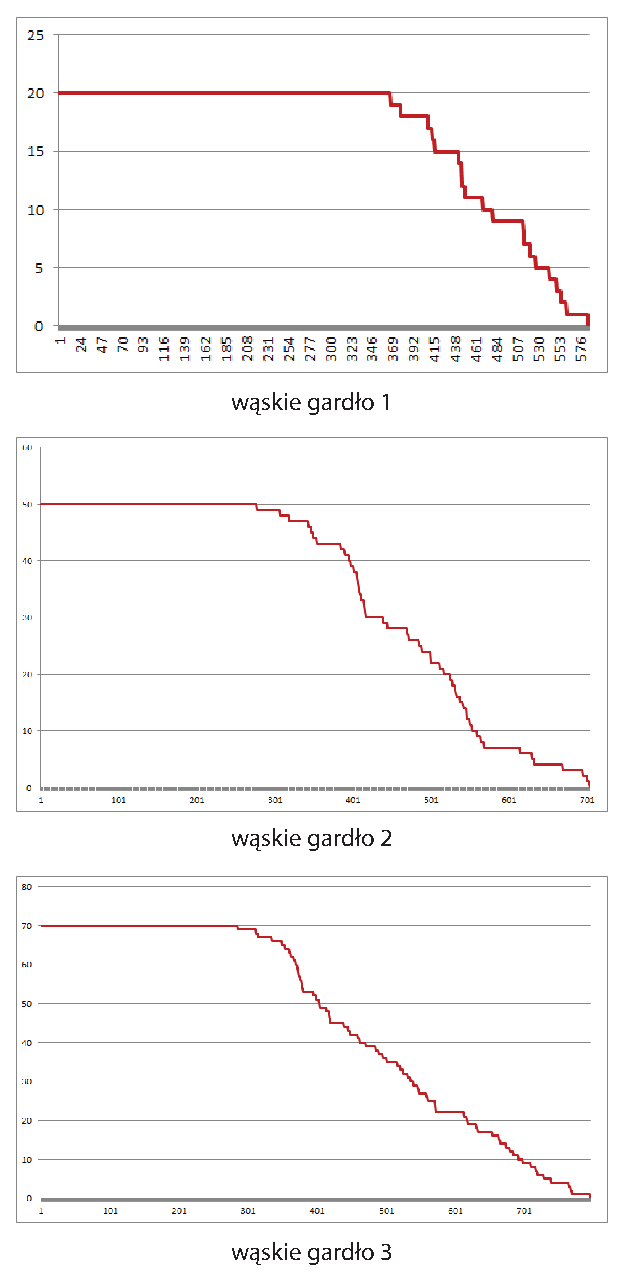
\includegraphics[width=0.4\textwidth]{iloscpieszychwaskie.eps}
\caption{Liczba pieszych w czasie - wąskie gardło}
\end{figure}
\end{samepage}

\begin{figure}
\label{figure:siatka}
\centering
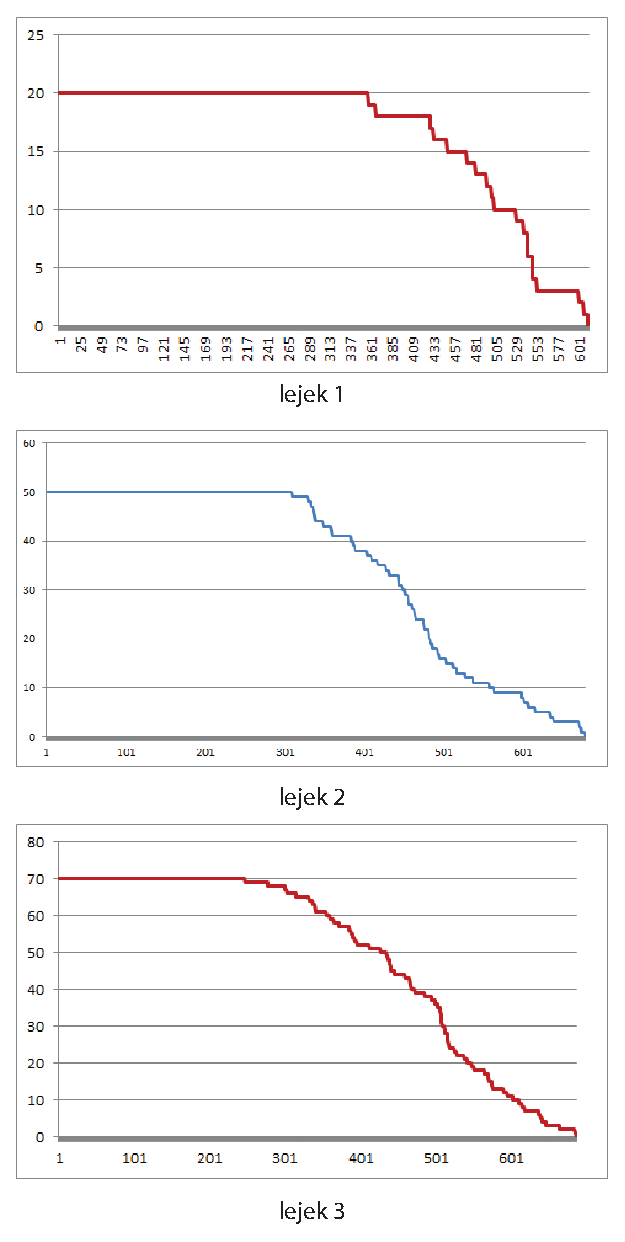
\includegraphics[width=0.5\textwidth]{iloscpieszychlejek.eps}
\caption{Liczba pieszych w czasie - lejek}
\end{figure}

\begin{figure}
\label{figure:siatka}
\centering
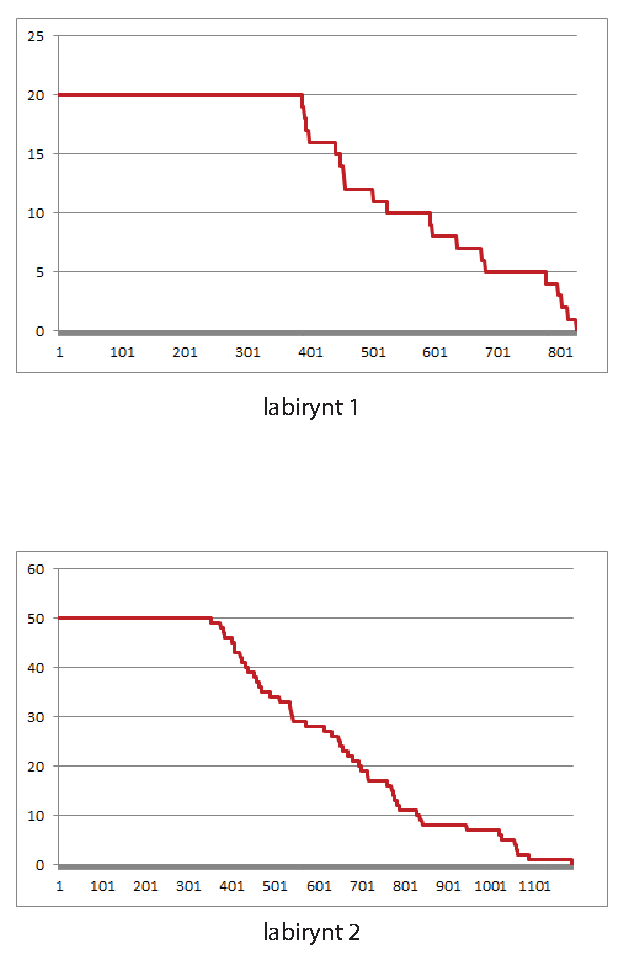
\includegraphics[width=0.5\textwidth]{iloscpieszychlabirynt.eps}
\caption{Liczba pieszych w czasie - labirynt}
\end{figure}

% \include{dodatekB}
% itd.

\printbibliography

\end{document}
